%% TEMPLATE PRESENTAZIONE BEAMER (tema Metropolis)
%%
%% Decision & Control Lab
%% Politecnico di Bari
%%
%% NON MODIFICARE i file nella cartella 00-settings.
%% Dichiarazione della classe e caricamento del tema (NON MODIFICARE)
\documentclass[10pt,xcolor={dvipsnames,svgnames,x11names}]{beamer}
\usetheme[block=fill,numbering=fraction,progressbar=frametitle]{metropolis}
\usepackage{00-settings/style}
%%%%%%%%%%%%%%%%%%%%%%%%%%%%%%%%%%%%%%%%%%%%%%%%%%%%%%%%%%%%%%%%%%%%%%%%%%%%%%%

%%%%%%%%%%%%%%%%%%%%%%%%%%%%%%%%%%%%%%%%%%%%%%%%%%%%%%%%%%%%%%%
% CONFIGURA QUI: tutte le informazioni della presentazione si
% cambiano modificando solo questo blocco, non serve toccare
% altri file.
%%%%%%%%%%%%%%%%%%%%%%%%%%%%%%%%%%%%%%%%%%%%%%%%%%%%%%%%%%%%%%%

% --- Titolo e sottotitolo (es. nome/luogo/data della conferenza) ---
\title{Title of the presentation}
\subtitle{Event, date, country.}

% --- Autori ---
% Nelle parentesi quadre va indicato l'autore che presenta (short author,
% usato in fondo alle slide); nelle graffe la lista completa degli autori.
\author[Mario Rossi (\url{mario.rossi@poliba.it})]{Anna~Bianchi\inst{1}, Mario~Rossi\inst{1}, Luca~Verdi\inst{2} \& Giulia Neri\inst{1}}

% --- Istituzioni/dipartimenti degli autori (\inst{n} li richiama sopra) ---
\institute{
\inst{1}Secret Lab of Experimental Stuff\\
University of Somewhere\and
\inst{2}Department of Stripy Confectioners\\
College of Somewhere Else}

% --- Data della presentazione ---
\date{April 21, 2022}

% --- Loghi in basso a destra su ogni slide (opzionale) ---
% Elenca i loghi separati da virgola: puoi metterne 1, 2, 3 o quanti
% vuoi, mettendo i file (png/jpg/pdf) nella cartella 00-settings.
% Per non mostrare alcun logo lascia la lista vuota: \renewcommand{\loghi}{}
\renewcommand{\loghi}{00-settings/LogoPoliBa.png,00-settings/LogoDandC.png,00-settings/dmmm.png}
%%%%%%%%%%%%%%%%%%%%%%%%%%%%%%%%%%%%%%%%%%%%%%%%%%%%%%%%%%%%%%%

%%%%%%%%% DOCUMENTO (contenuto delle slide, modificare liberamente) %%%%%%%%%
\begin{document}

\begin{frame}[noframenumbering,plain]
\titlepage
\end{frame}

\begin{frame}{Table of contents}
  \setbeamertemplate{section in toc}[sections numbered]
  \tableofcontents%[hideallsubsections]
\end{frame}

\section[Intro]{Introduction}

\begin{frame}[fragile]{Sections}
  Sections group slides of the same topic

  \begin{verbatim}    \section{Elements} \end{verbatim}
  
\end{frame}

\section{Titleformats}

\begin{frame}{Small caps}

	\begin{alertblock}{Potential Problems}
		Be aware, that not every font supports small caps. If for example you typeset your presentation with pdfTeX and the Computer Modern Sans Serif font, every text in smallcaps will be typeset with the Computer Modern Serif font instead.
	\end{alertblock}

 	\begin{exampleblock}{Potential Problems}
 	    		Be aware, that not every font supports small caps. If for example you typeset your presentation with pdfTeX and the Computer Modern Sans Serif font, every text in smallcaps will be typeset with the Computer Modern Serif font instead.
 	\end{exampleblock}
\end{frame}


\section{Elements}

\begin{frame}[fragile]{Typography}
      \begin{verbatim}The theme provides sensible defaults to
\emph{emphasize} text, \alert{accent} parts
or show \textbf{bold} results.\end{verbatim}

  \begin{center}becomes\end{center}

  The theme provides sensible defaults to \emph{emphasize} text,
  \alert{accent} parts or show \textbf{bold} results.
\end{frame}

\begin{frame}{Font feature test}
  \begin{itemize}
    \item Regular
    \item \textit{Italic}
    \item \textsc{SmallCaps}
    \item \textbf{Bold}
    \item \textbf{\textit{Bold Italic}}
    \item \textbf{\textsc{Bold SmallCaps}}
    \item \texttt{Monospace}
    \item \texttt{\textit{Monospace Italic}}
    \item \texttt{\textbf{Monospace Bold}}
    \item \texttt{\textbf{\textit{Monospace Bold Italic}}}
  \end{itemize}
\end{frame}

\begin{frame}{Lists}
  \begin{columns}[T,onlytextwidth]
    \column{0.45\textwidth}
      Items
      \begin{itemize}
        \item Milk 
        \item Eggs 
        \item Potatos
      \end{itemize}

    \column{0.45\textwidth}
      Enumerations
      \begin{enumerate}
        \item First, 
        \item Second and 
        \item Last.
      \end{enumerate}
  \end{columns}
\end{frame}

\begin{frame}{Animation}
  \begin{itemize}[<+- | alert@+>]
    \item \alert<4>{This is\only<4>{ really} important}
    \item Now this
    \item And now this
  \end{itemize}
\end{frame}

\begin{frame}{Tables}
  \begin{table}
    \caption{Largest cities in the world (source: Wikipedia)}
    \begin{tabular}{lr}
      \toprule
      City & Population\\
      \midrule
      Mexico City & 20,116,842\\
      Shanghai & 19,210,000\\
      Peking & 15,796,450\\
      Istanbul & 14,160,467\\
      \bottomrule
    \end{tabular}
  \end{table}
\end{frame}
\begin{frame}{Figures}
  Images go in 02-figures and are included as usual with \texttt{\textbackslash includegraphics}.
  \begin{figure}
    \centering
    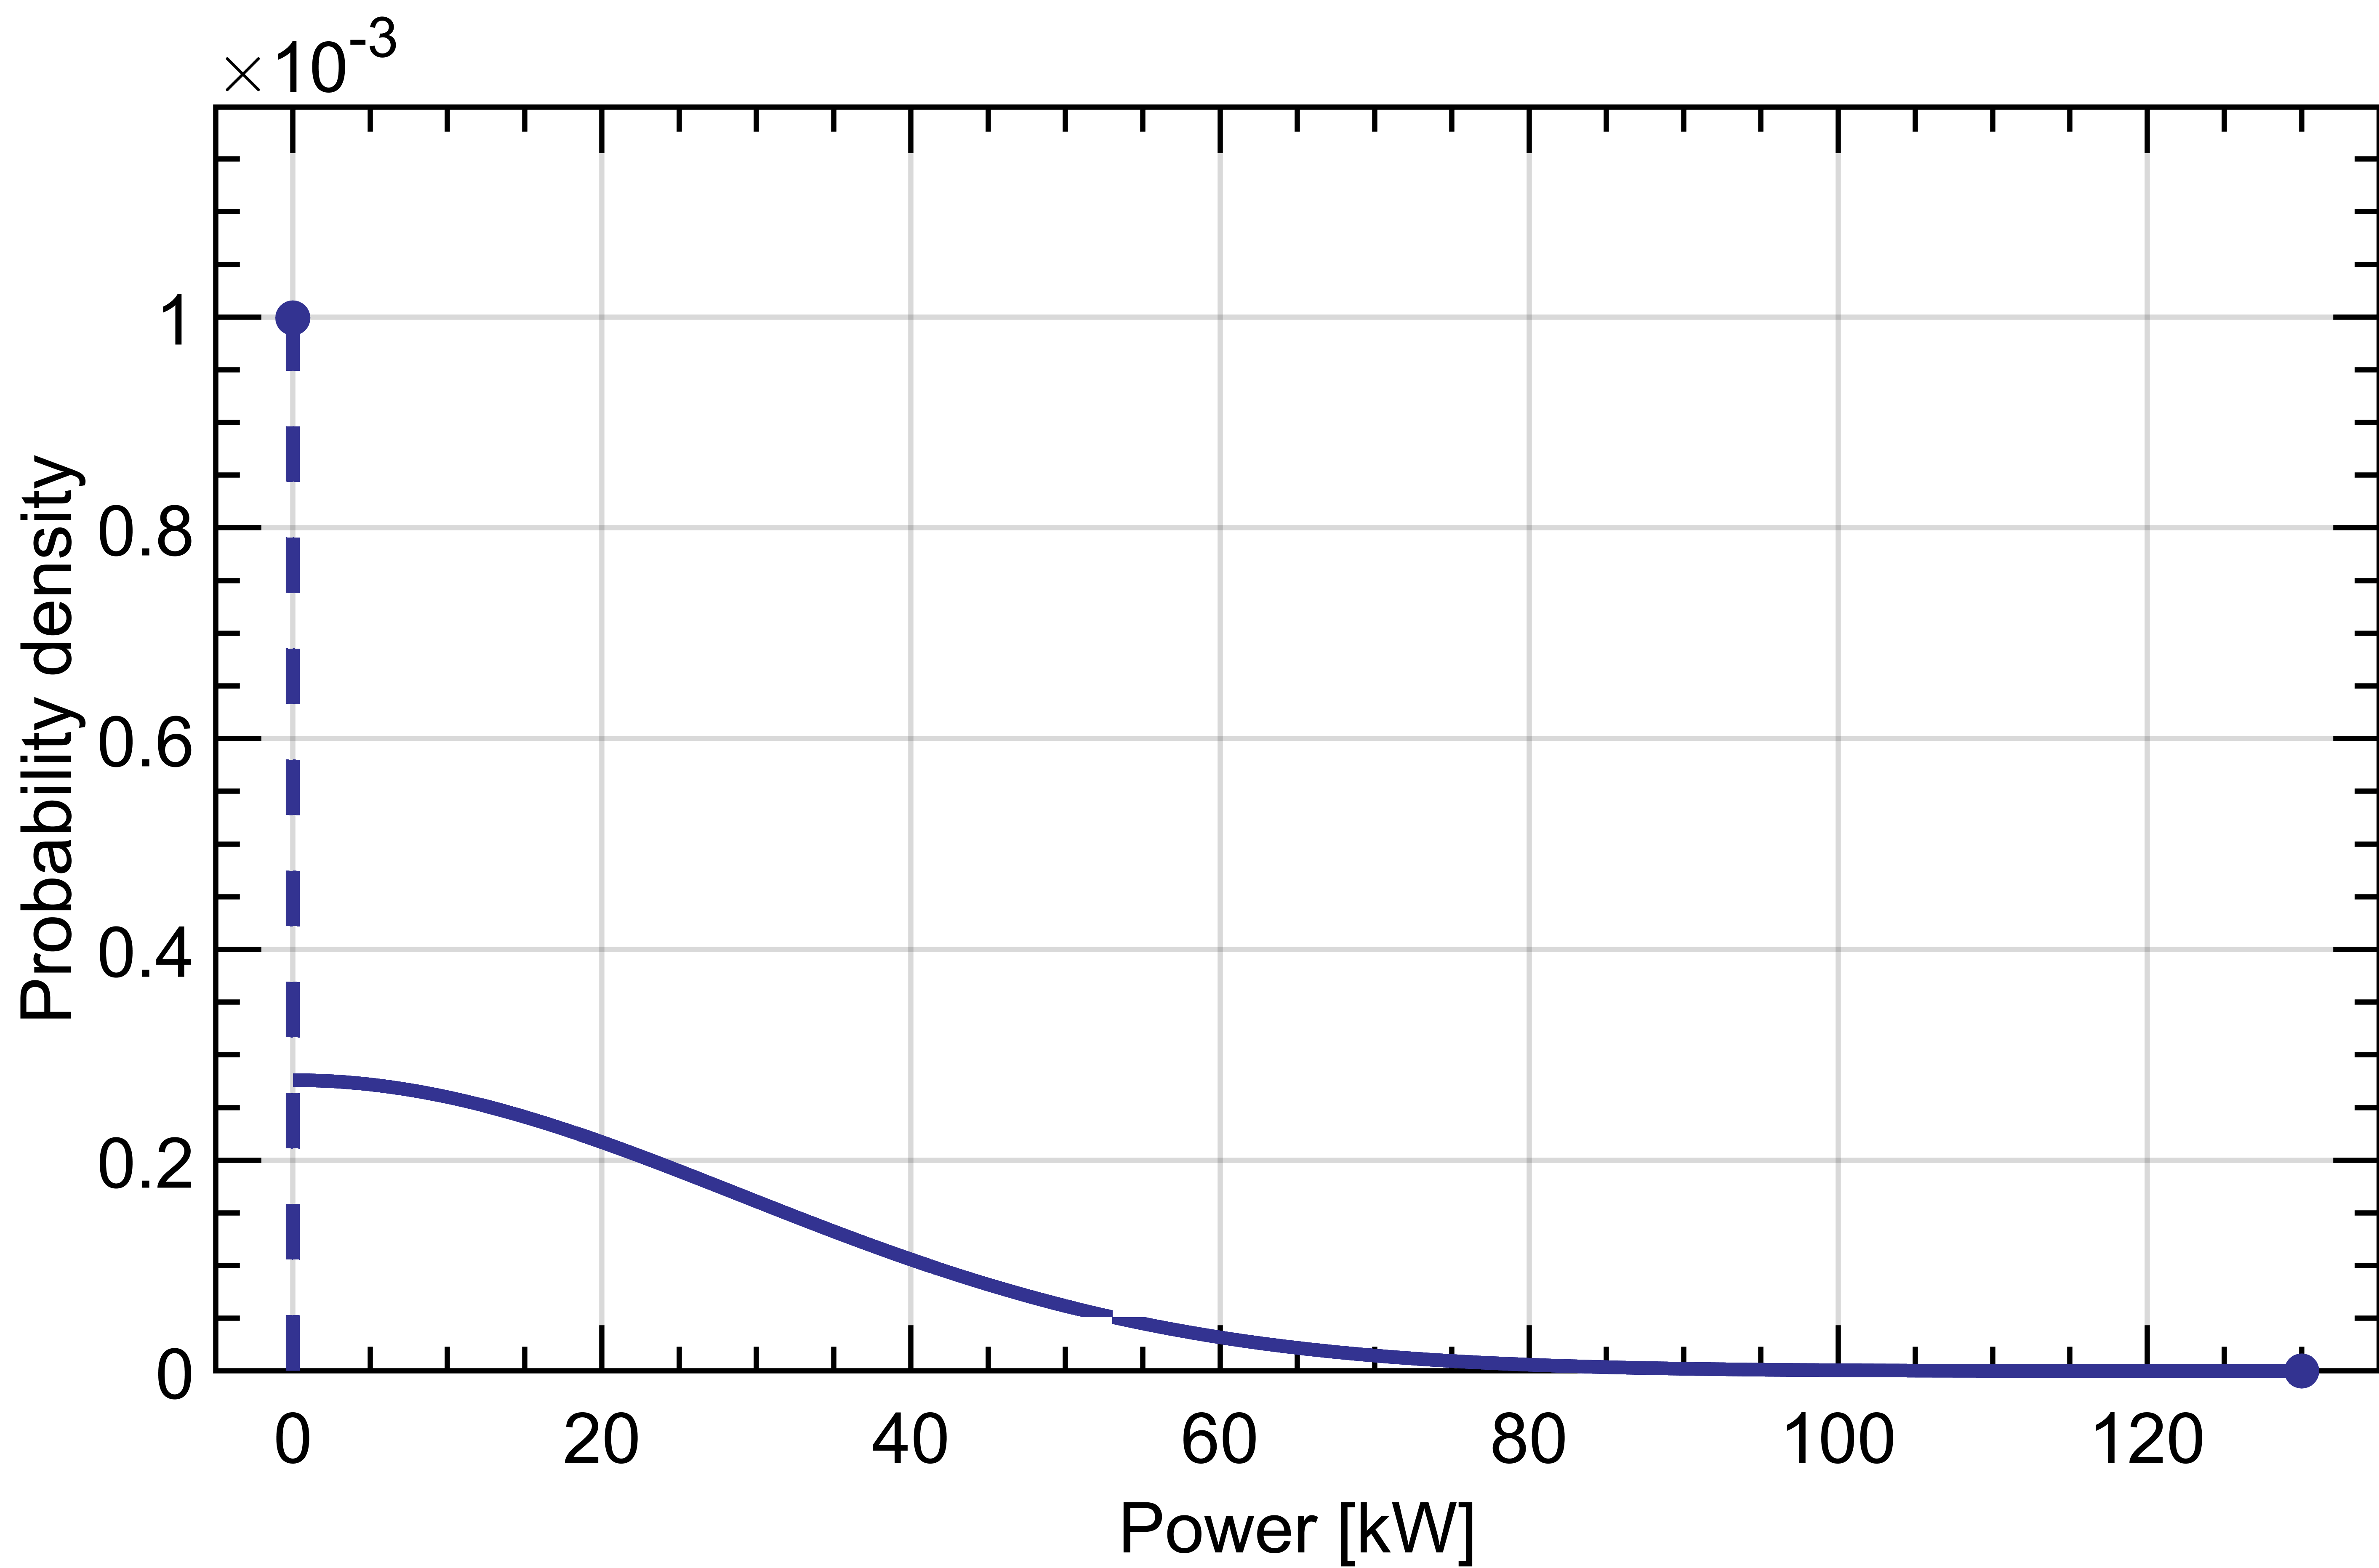
\includegraphics[width=0.5\textwidth]{02-figures/esempioFigura.png}
    \caption{Example figure.}
  \end{figure}
\end{frame}

\begin{frame}[fragile]{Code}
  Source code lives in 03-code, in a subfolder per language (Matlab or Python).

  \begin{columns}[T,onlytextwidth]
    \column{0.45\textwidth}
      \small Matlab (\texttt{mcode} style):
      \lstinputlisting[basicstyle=\tiny\ttfamily,firstline=1,lastline=8]{03-code/matlab/Codice1.m}
    \column{0.45\textwidth}
      \small Python (\texttt{pythonstyle}):
      \lstinputlisting[style=pythonstyle,basicstyle=\tiny\ttfamily,firstline=1,lastline=8]{03-code/python/Codice1.py}
  \end{columns}
\end{frame}

\begin{frame}{Blocks}
  Three different block environments are pre-defined and may be styled with an
  optional background color.

      \begin{block}{Default}
        Block content.
      \end{block}

      \begin{alertblock}{Alert}
        Block content.
      \end{alertblock}

      \begin{exampleblock}{Example}
        Block content.
      \end{exampleblock}
      
\end{frame}
\begin{frame}{Math}
  \begin{equation*}
    e = \lim_{n\to \infty} \left(1 + \frac{1}{n}\right)^n
  \end{equation*}
\end{frame}

\begin{frame}{References}
  Some references to showcase \cite{kim2015coordination,carli2020energy}
\end{frame}

\section{Conclusion}


{\setbeamercolor{palette primary}{fg=black, bg=white}
\begin{frame}[standout]
  Questions?
\end{frame}
}

\appendix

\begin{frame}[fragile]{Backup slides}
  Sometimes, it is useful to add slides at the end of your presentation to
  refer to during audience questions.

  The best way to do this is to include the \verb|appendixnumberbeamer|
  package in your preamble and call \verb|\appendix| before your backup slides.

\end{frame}

\begin{frame}[allowframebreaks]{References}

  \bibliography{references}
  \bibliographystyle{abbrv}
\end{frame}
\end{document}
